\documentclass{article}
\usepackage[xetex]{graphicx}
\usepackage{fontspec,xunicode}
\defaultfontfeatures{Mapping=tex-text,Scale=MatchLowercase}
\setmainfont[Scale=.95]{Calluna}
\setmonofont{Lucida Sans Typewriter}



\usepackage{xltxtra}
%\fontspec[Path = /Users/tvooo/Library/Fonts/]{SourceCodePro-Regular.otf}

%\setmainfont[
%  Extension = .otf,
%  UprightFont = *-regular,
%  BoldFont = *-bold,
%  ItalicFont = *-italic,
%  BoldItalicFont = *-bolditalic,
%]{SourceCodePro}

\begin{document}

\title{A Sample \LaTeX{} Document}
\author{Tim von Oldenburg}

\maketitle

\begin{abstract}
The abstract text goes here.
\end{abstract}

\section{Introduction}
Here is some introductory copy.
Lorem ipsum dolor sit amet, consectetur adipisicing elit, sed do eiusmod
tempor incididunt ut labore et dolore magna aliqua. Ut enim ad minim veniam,
quis nostrud exercitation ullamco laboris nisi ut aliquip ex ea commodo
consequat. Duis aute irure dolor in reprehenderit in voluptate velit esse
cillum dolore eu fugiat nulla pariatur. Excepteur sint occaecat cupidatat non
proident, sunt in culpa qui officia deserunt mollit anim id est laborum.

\begin{equation}
    \label{simple_equation}
    \alpha = \sqrt{ \beta }
\end{equation}

\subsection{Subsection Heading Here}
Write your subsection text here.

\begin{figure}
    \centering
    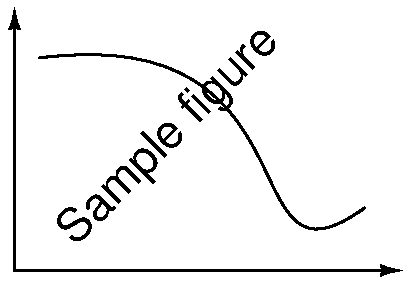
\includegraphics[width=3.0in]{figure}
    \caption{Simulation Results}
    \label{simulationfigure}
\end{figure}

\section{Conclusion}
Write your conclusion here.

\end{document}


